\documentclass[tikz,border=10pt]{standalone}
\usepackage[scaled=0.95]{helvet}
\renewcommand{\familydefault}{\sfdefault}
\usepackage{tikz}
\usetikzlibrary{arrows.meta,positioning}
\definecolor{TEJNavy}{HTML}{1E2B55}
\definecolor{TEJBlue}{HTML}{1769AA}
\definecolor{TEJGreen}{HTML}{2B7A53}
\definecolor{TEJGold}{HTML}{D49B19}
\definecolor{TEJRed}{HTML}{A43737}
\definecolor{TEJLight}{HTML}{EEF6F8}
\begin{document}
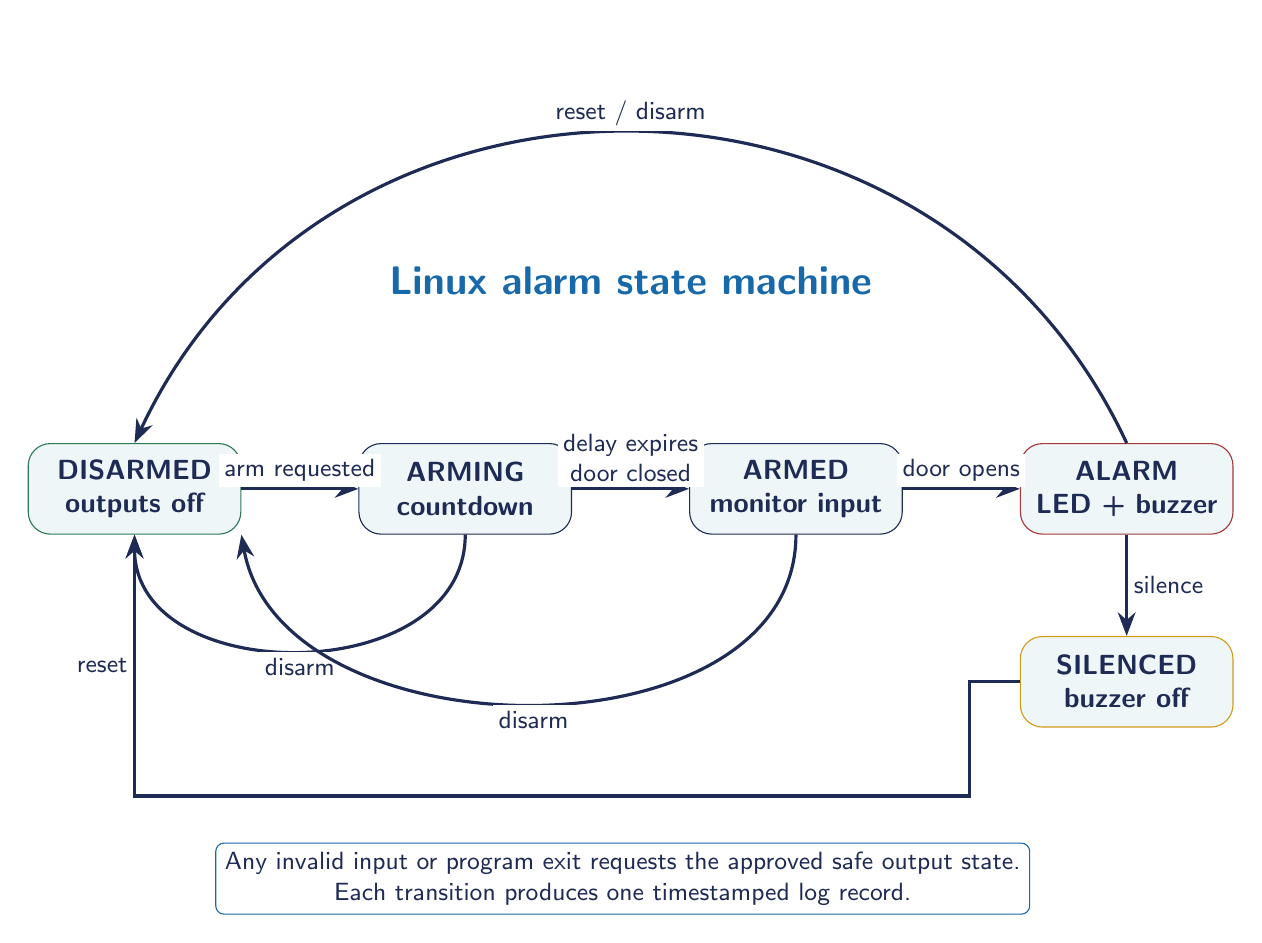
\begin{tikzpicture}[
  font=\sffamily,
  text=TEJNavy,
  state/.style={draw=TEJNavy,rounded corners=8pt,fill=TEJLight,minimum width=2.7cm,minimum height=1.15cm,align=center,font=\bfseries},
  arrow/.style={-{Stealth[length=3mm]},line width=1.15pt,draw=TEJNavy},
  note/.style={font=\small,align=center,fill=white,inner sep=2pt}
]
  \node[font=\bfseries\Large,text=TEJBlue] at (8.1,7.45)
    {Linux alarm state machine};

  \node[state,draw=TEJGreen] (disarmed) at (1.8,4.8) {DISARMED\\outputs off};
  \node[state] (arming) at (6.0,4.8) {ARMING\\countdown};
  \node[state] (armed) at (10.2,4.8) {ARMED\\monitor input};
  \node[state,draw=TEJRed] (alarm) at (14.4,4.8) {ALARM\\LED + buzzer};
  \node[state,draw=TEJGold] (silenced) at (14.4,2.35) {SILENCED\\buzzer off};

  \draw[arrow] (disarmed) -- node[note,above]{arm requested} (arming);
  \draw[arrow] (arming) -- node[note,above]{delay expires\\door closed} (armed);
  \draw[arrow] (armed) -- node[note,above]{door opens} (alarm);
  \draw[arrow] (alarm) -- node[note,right]{silence} (silenced);

  \draw[arrow] (arming.south) to[out=-90,in=-90,looseness=1.2]
    node[note,below]{disarm} (disarmed.south);
  \draw[arrow] (armed.south) to[out=-90,in=-80,looseness=1.05]
    node[note,below]{disarm} (disarmed.south east);
  \draw[arrow] (alarm.north) to[out=115,in=65,looseness=1.18]
    node[note,above]{reset / disarm} (disarmed.north);
  \draw[arrow] (silenced.west) -- (12.4,2.35) -- (12.4,0.9) -- (1.8,0.9) --
    node[note,left]{reset} (disarmed.south);

  \node[draw=TEJBlue,rounded corners=3pt,align=center,font=\small]
    at (8.0,-0.15) {Any invalid input or program exit requests the approved safe output state.\\Each transition produces one timestamped log record.};
\end{tikzpicture}
\end{document}
